\documentclass[border=0.5in]{blog}


\usetikzlibrary{arrows,shapes,snakes,automata,backgrounds,petri,matrix,shapes.multipart,    positioning,shapes.callouts,shapes.arrows,calc}

\tikzstyle{brick} = [rectangle, minimum height = 0.7cm, text centered, draw = black]

\title{Notes for OctNet}
\author{Johann Lee \\ me@qinka.pro}
\date{Dec. 20, 2017}

\newcommand\drawbox[2]{
    \draw [draw=black,shift={#1}] (-#2,-#2) -- (#2,-#2) -- (#2,#2) -- (-#2,#2) -- (-#2,-#2)}
\newcommand\drawcross[3]{%
    \draw [draw=black] (#1-#3,#2) -- (#1+#3,#2);
    \draw [draw=black] (#1,#2-#3) -- (#1,#2+#3)
}
\newcommand\drawcrosssym[3]{%
    \drawcross{-#1}{-#2}{#3};
    \drawcross{-#1}{#2}{#3};
    \drawcross{#1}{-#2}{#3};
    \drawcross{#1}{#2}{#3}
}

\begin{document}
    
    \maketitle
    
    \begin{abstract}
        This post is the notes about a Octree-based 3-D convolutional neural network, presented by
        \citep{DBLP:journals/tog/WangLGST17} in \textit{O-CNN: Octree-based Convolutional Neural Networks for 3D Shape Analysis}.
    \end{abstract}

    \tableofcontents
    
    \section{Data Structure of O-CNN}
    \label{sec:o-cnn-ds}
    
    In the \citep{DBLP:journals/tog/WangLGST17}, the primary items of O-CNN is the data structure,
    and how do the computing of tensor-based operational do use the octree-based data.
    This section is about the data structure of O-CNN.
    
    The O-CNN include four tables primarily, and three of them is:
    \textit{shuffled key table}, \textit{label table}, and \textit{feature vector(table)}.
    The continuous arrays, \textit{feature vector}, is to pack the features and data of
    sparse octants at each depth. Label buffer, or say label table, is to fetch the correspondence
    between the features at different levels so that the convolutional operations can be computed
    efficiently.
    
    \subsection{Shuffled Key}
    \label{sec:o-cnn-ds:sk}
    
    The shuffled keys is a key to encode the an octant's location at depth $l$.
    That can be recursively defined, just like Eq..
    \begin{equation}
        \label{eq:shuffled-key-rec}
        key\left(O\right) = key\left(parent\left(O\right)\right):x_ly_lz_l
    \end{equation}
    where $:$ denotes connecting. For example, there is a octant $O$ located at $(x,y,z)$.
    The $x_1x_2\dots x_l$ is the binary number of $x$, and in the similar way, there are also
    $y_1y_2\dots y_l$ and $z_1z_2\dots z_l$. The shuffled key of $O$ will be $x_1y_1z_1x_2y_2z_2\dots x_ly_lz_l$. Meanwhile, the shuffled key is also the index of octant
    in the $l$ depth tables, while the shuffled key table, label table, and feature vector share 
    the same index of a octant.
    
    \subsection{Label}
    \label{sec:o-cnn-ds:l}
    
    So the label is another important thing. The labels is the data index of the octant.
    For the octant $O$ at depth $l$, the data of $O$ is $L_{(l)}\left[S_{(l)}\left[O\right]\right]$.
    In other word,the table of labels at depth $l$, $L_(l)$ store the index of octant $O$ in feature vector.
    
    The first index in table is $1$, not $0$, while the empty octant's index is $0$.
    So that we can store $0$ in the location whose index is $0$.
    Moreover, the table of label can also describe the shape of octree,
    because the index of node which is the finest leaf-node and do not have sub-nodes is $0$.
    
    \subsection{Feature vector(table)}
    \label{sec:o-cnn-d:fv}
    
    The feature vectors hold two things: feature computed by CNN, and data of octant.
    The $T_{(l)}$ store the feature, while the data input vector store the original input data.
    
    \subsection{Super-octree: Mini-batch of 3D models}
    \label{sec:o-cnn-d:so}
    
    Because the data is sparse and the shapes of different object are different,
    there are a problem and a solution. The problem is that it is hard and non-efficient that
    do the O-CNN operations on a batch with many different object.
    However, when the objects in different shapes mounted into a single super-octree,
    these objects will be regarded as single object, and the computing can be computed efficiently.
    
    \subsection{Hash table}
    \label{sec:o-cnn-d:ht}
    
    With above data structures, the convolutional operations can be done with the tensor-based
    convolutional operations. However, the operation of find the location of a octant in $S$,
    it not efficient. \citep{DBLP:journals/tog/WangLGST17} present a hash table to get the location
    quickly.
    
    By the way, they also mention that for the convolution, the hash table some times share the
    neighbors so that the searching time can be reduced.
    
            
    \subsection{Example}
    \label{sec:o-cnn-ds:eg}
    
    In this section, I will try to use an example to explain these elements in O-CNN.
    The example is based on Fig.\ref{fig:eg1:circle:circle}, and it is a 2-D sparse image with quad-tree, just like \ref{fig:eg1:circle:co}.
    \begin{figure}
        \centering
        \subfigure[A circle with grid]{
        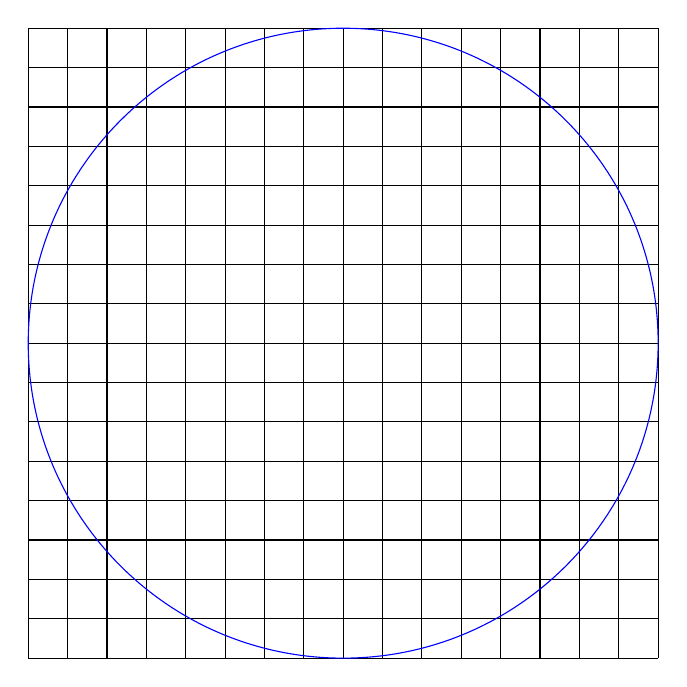
\begin{tikzpicture}
            \draw[step=0.5cm] (-4,-4) grid (4,4);  
            \draw[color = blue]circle(4cm);
        \end{tikzpicture}
        \label{fig:eg1:circle:circle}}
        \subfigure[Represented with quad-tree]{
        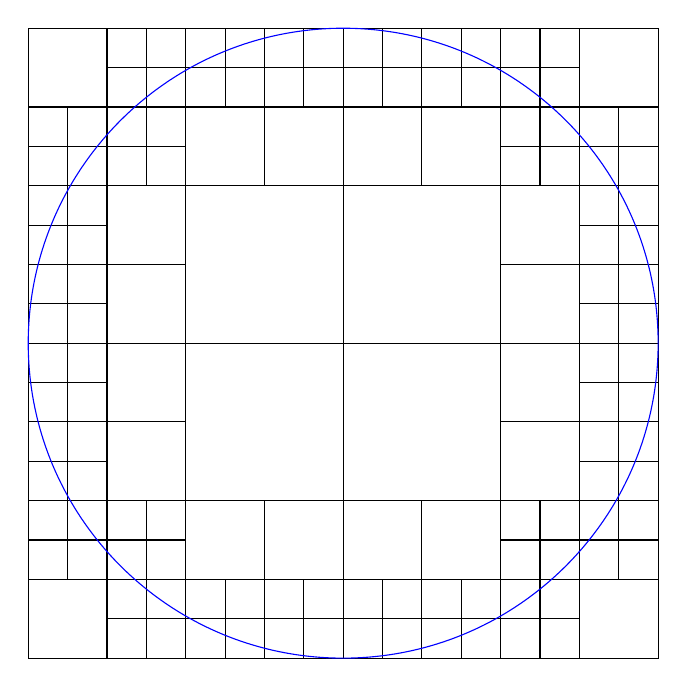
\begin{tikzpicture}
            \drawbox{(0,0)}{4};
            \drawcross{0}{0}{4};
            \drawcrosssym{2}{2}{2};
            \drawcrosssym{3}{3}{1};
            \drawcrosssym{1}{3}{1};
            \drawcrosssym{3}{1}{1};
            \drawcrosssym{3.5}{2.5}{0.5};
            \drawcrosssym{2.5}{3.5}{0.5};
            \drawcrosssym{2.5}{2.5}{0.5};
            \drawcrosssym{1.5}{3.5}{0.5};
            \drawcrosssym{0.5}{3.5}{0.5};
            \drawcrosssym{3.5}{1.5}{0.5};
            \drawcrosssym{3.5}{0.5}{0.5};
            \draw[color = blue]circle(4cm);
        \end{tikzpicture}
        \label{fig:eg1:circle:co}}
        \caption{A circle.}
        \label{fig:eg1:circle}
    \end{figure}
    
    
    \subsubsection{Shuffled Key}
    \label{sec:o-cnn-d:eg:sk}
    
    As Fig.\ref{fig:eg1:circle:co} shown, the image includes 5 levels, or say the depth of 
    image is 5, from level $l_0$ to $l_4$. So the vector of each level should be looked like
    the 
    
    \begin{figure}
        \centering
        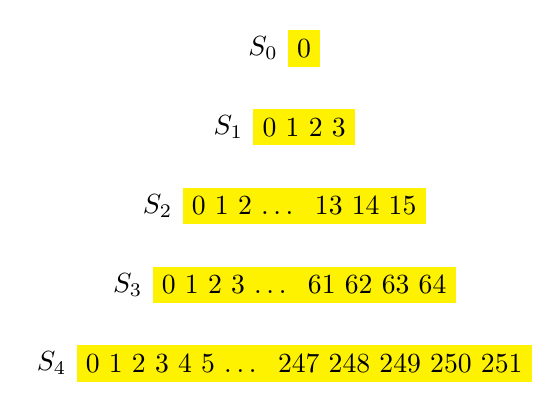
\begin{tikzpicture}
        \node[fill=yellow,align=center]
        (s0) {0};
        \node[anchor=east] at (s0.west) {$S_0$};
        \node[fill=yellow,align=center,below of=s0]
        (s1) {0 1 2 3};
        \node[anchor=east] at (s1.west) {$S_1$};
        \node[fill=yellow,align=center,below of=s1]
        (s2) {0 1 2 \dots\, 13 14 15};
        \node[anchor=east] at (s2.west) {$S_2$};
        \node[fill=yellow,align=center,below of=s2]
        (s3) {0 1 2 3 \dots\, 61 62 63 64};
        \node[anchor=east] at (s3.west) {$S_3$};
        \node[fill=yellow,align=center,below of=s3]
        (s4) {0 1 2 3 4 5 \dots\, 247 248 249 250 251};
        \node[anchor=east] at (s4.west) {$S_4$};
        \end{tikzpicture}
        \caption{Tables of shuffled keys}
        \label{fig:o-cnn-d:eg:sk}
    \end{figure}
    
    There are 48 items in $S_{(3)}$, but some of them is not continuous, because some octant in
    depth $2$ do not have sub-nodes, and the shuffled key is make up with the information of location. In same case, the $S_{(4)}$ have 111 items.
    
    \paragraph{Label table}
    
    Then we can get the label table. As everybody known, the $L_{(0)}$ only has a element,
    and it is zero, just like Fig.\ref{fig:o-cnn-d:eg:l}, while $L_{(1)}$, $L_{(2)}$, $L_{(3)}$
    and $L_{(4)}$ also have some items, and some of them is $0$.
    
    For $L_{(4)}$, there are 111 item, and only 60 of them is non-zero.
    
    \begin{figure}
        \centering
        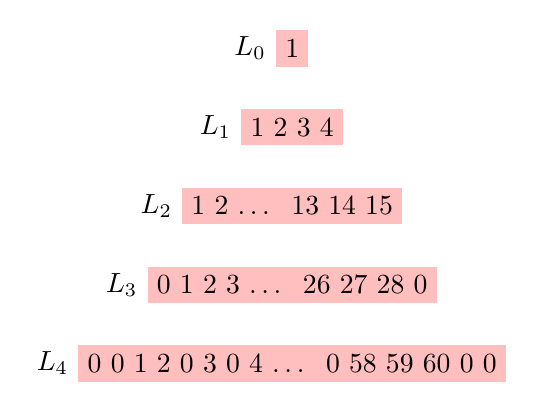
\begin{tikzpicture}
            \node[fill=pink,align=center]
            (l0) {1};
            \node[anchor=east] at (l0.west) {$L_0$};
            \node[fill=pink,align=center,below of=l0]
            (l1) {1 2 3 4};
            \node[anchor=east] at (l1.west) {$L_1$};
            \node[fill=pink,align=center,below of=l1]
            (l2) {1 2 \dots\, 13 14 15};
            \node[anchor=east] at (l2.west) {$L_2$};
            \node[fill=pink,align=center,below of=l2]
            (l3) {0 1 2 3 \dots\, 26 27 28 0};
            \node[anchor=east] at (l3.west) {$L_3$};
            \node[fill=pink,align=center,below of=l3]
            (l4) {0 0 1 2 0 3 0 4 \dots\, 0 58 59 60 0 0};
            \node[anchor=east] at (l4.west) {$L_4$};
        \end{tikzpicture}
        \caption{Tables of labels}
        \label{fig:o-cnn-d:eg:l}
    \end{figure}
    
    
    \subsubsection{Feature Vector \& Input Signal}
    \label{sec:o-cnn-d:eg:fvnis}
    
    The vector of input signal should be like Fig.\ref{fig:o-cnn-d:eg:vis}.
    
    \begin{figure}
        \centering
        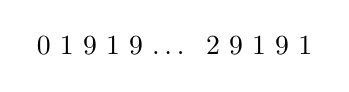
\begin{tikzpicture}
            \node[align=center]
            (l4) {0 1 9 1 9 \dots\, 2 9 1 9 1};
        \end{tikzpicture}
        \caption{Vector of input signal}
        \label{fig:o-cnn-d:eg:vis}
    \end{figure}
    
    Then we can do the convolution operation, and the feature vector of depth $4$ will be like
    Fig.\ref{fig:o-cnn-d:eg:fv4}.
    
    \begin{figure}
        \centering
        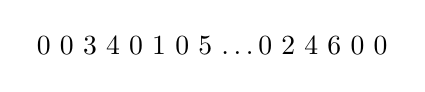
\begin{tikzpicture}
        \node[align=center]
        (l4) {0 0 3 4 0 1 0 5 \dots 0 2 4 6 0 0};
        \end{tikzpicture}
        \caption{Feature vector for depth $4$}
        \label{fig:o-cnn-d:eg:fv4}
    \end{figure}

    Then we can do the pooling operation, and the feature vector of depth $3$ will be like Fig.\ref{fig:o-cnn-d:eg:fv3}.
    
    \begin{figure}
        \centering
        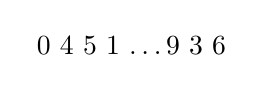
\begin{tikzpicture}
        \node[align=center]
        (l4) {0 4 5 1 \dots 9 3 6};
        \end{tikzpicture}
        \caption{Feature vector for depth $3$}
        \label{fig:o-cnn-d:eg:fv3}
    \end{figure}
    
    \section{How does it work?}
    \label{sec:o-cnn-work}
    
    The convolutional operations of O-CNN is tensor-based, so that the key point of O-CNN is
    transformation between the euclidean index $(i,j,k)$ and the octree index $index(O)$.
    The shuffled key $key(O)$ is encoded according to euclidean location, so the transformation
    between shuffled key and euclidean index can be easily established. With the shuffled key table $S$
    the relationship between shuffled key and index can also be established. However the latter
    is not as easy as the former.
    
    To establish relationship easily, O-CNN use the hash table 
    $$
        H:key(O) \mapsto index(O)
    $$ 
    However, the hash table is not as efficient as we want. The sibling nodes share the neighbors,
    So we can use the shared and pre-compiled hash-table to help to establish the relationship
    between $key(O)$ and $index(O)$.

    \bibliography{../../../random-bib/2-D-CNN%
        ,../../../random-bib/3d-deep-learning%
        %
    }

    \bibliographystyle{plainnat}    
\end{document}
